%
% Capítulo 3
%
\chapter{Solução do Problema} \label{cap3}

\section{Modelo de Dados}\label{sec31}

% Modelo EA
\subsection{Modelo Entidade-Associação}

\begin{figure}
	\centering
	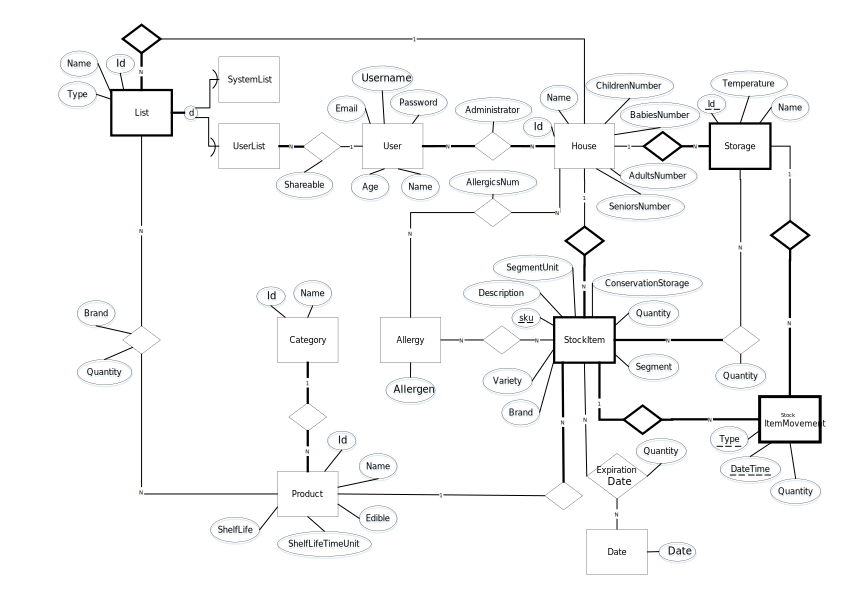
\includegraphics[width=20cm,height=16cm,scale=0.5]{./files/EA.pdf}
	\caption{Modelo Entidade-Associação}
	\label{modelo-ea}
\end{figure}

% Modelo Relacional
\subsection{Modelo Relacional}
{\parindent 0pt
	\begin{description}
		\item House(house\_id, house\_name, house\_babiesNumber, house\_childrenNumber, house\_adultsNumber, house\_seniorsNumber) \newline
		\acrshort{cp}: (house\_id) 
		
		\item User(user\_username, user\_email, user\_age, user\_name, user\_password) \newline
		\acrshort{cp}: (user\_username)  \newline
		\acrshort{occ}: (user\_email)
		
		\item Allergy(allergy\_allergen) \newline
		\acrshort{cp}: (allergy\_allergen) 
		
		\item Recipe(recipe\_id, recipe\_name, recipe\_instructions, recipe\_difficulty, recipe\_time, recipe\_servings, recipe\_cuisine, recipe\_dishType, recipe\_type) \newline
		\acrshort{cp}: (recipe\_id) 
		
		\item SystemRecipe(recipe\_id) \newline
		\acrshort{cp}: (recipe\_id) \newline
		\acrshort{ce}: \{(recipe\_id) ref Recipe\}
		
		\item UserRecipe(recipe\_id, user\_username) \newline
		\acrshort{cp}: (recipe\_id) \newline
		\acrshort{ce}: \{(recipe\_id) ref Recipe, (user\_username) ref User\}
		
		\item SharedRecipe(recipe\_id, user\_username) \newline
		\acrshort{cp}:(recipe\_id, user\_username) \newline
		\acrshort{ce}: \{(recipe\_id) ref UserRecipe, (user\_username) ref User\}
		
		\item List(house\_id, list\_id, list\_name, list\_type) \newline
		\acrshort{cp}: (house\_id, list\_id) \newline
		\acrshort{ce}: \{(house\_id) ref House\}
		
		\item SystemList(house\_id, list\_id)
		\newline
		\acrshort{cp}: (house\_id, list\_id) \newline
		\acrshort{ce}: \{(house\_id, list\_id) ref List\}
		
		\item UserList(house\_id, list\_id, user\_username, list\_shareable)
		\newline
		\acrshort{cp}: (house\_id, list\_id) \newline
		\acrshort{ce}: \{(house\_id, list\_id) ref List, (user\_username) ref User\}
		
		\item Category(category\_id, category\_name)
		\newline
		\acrshort{cp}: (category\_id) \newline
		\acrshort{occ}: (category\_name)
		
		\item Product(category\_id, product\_id, product\_name, product\_edible, product\_shelfLife, \newline product\_shelfLifeTimeUnit) \newline
		\acrshort{cp}: (category\_id, product\_id) \newline
		\acrshort{ce}: \{(category\_id) ref Category\}
		
		\item StockItem(house\_id, stockItem\_sku, category\_id, product\_id, stockItem\_brand, stockItem\_segment, stockItem\_variety, stockItem\_quantity, stockItem\_segmentUnit, stockItem\_description, stockItem\_conservationStorage) \newline
		\acrshort{cp}: (house\_id, stockItem\_sku) \newline
		\acrshort{occ}: (house\_id, category\_id, product\_id, stockItem\_brand, stockItem\_segment, \newline stockItem\_variety) \newline
		\acrshort{ce}: \{(house\_id) ref House, (category\_id, product\_id) ref Product\}
		
		\item Ingredient(recipe\_id, category\_id, product\_id, ingredient\_quantity, ingredient\_quantityUnit) \newline
		\acrshort{cp}: (recipe\_id, category\_id, product\_id) \newline
		\acrshort{ce}: \{(recipe\_id) ref Recipe, (category\_id, product\_id) ref Product\}
		
		\item Storage(house\_id, storage\_id, storage\_name, storage\_temperature)  \newline
		\acrshort{cp}:(house\_id, storage\_id) \newline
		\acrshort{ce}: \{(house\_id) ref House\}
	
		\item UserHouse(house\_id, user\_username, userHouse\_administrator) \newline
		\acrshort{cp}: (house\_id, user\_username) \newline
		\acrshort{ce}: \{(house\_id) ref House, (user\_username) ref User\}
		
		\item StockItemStorage(house\_id, stockItem\_sku, storage\_id, stockItemStorage\_quantity) \newline
		\acrshort{cp}: (house\_id, stockItem\_sku, storage\_id) \newline
		\acrshort{ce}: \{(house\_id, stockItem\_sku) ref StockItem, (house\_id, storage\_id) ref Storage\}
		
		\item StockItemMovement(house\_id, stockItem\_sku, storage\_id, stockItemMovement\_type, \newline stockItemMovement\_dateTime, StockItemMovement\_quantity) \newline
		\acrshort{cp}: (house\_id, stockItem\_sku, storage\_id, stockItemMovement\_type, \newline stockItemMovement\_dateTime, StockItemMovement\_quantity) \newline
		\acrshort{ce}: \{(house\_id, stockItem\_sku) ref StockItem, (house\_id, storage\_id) ref Storage\}
		
		\item HouseAllergy(house\_id, allergy\_allergen, houseAllergy\_alergicsNum) \newline
		\acrshort{cp}: (house\_id, allergy\_allergen) \newline
		\acrshort{ce}: \{(house\_id) ref House, (allergy\_allergen) ref Allergy\}
	
		\item ListProduct(house\_id, list\_id, category\_id, product\_id, listProduct\_brand, listProduct\_quantity) \newline
		\acrshort{cp}: (house\_id, list\_id, category\_id, product\_id) \newline
		\acrshort{ce}: \{(house\_id, list\_id) ref List, (category\_id, product\_id) ref Product\}
	
		\item StockItemAllergy(house\_id, stockItem\_sku, allergy\_allergen) \newline
		\acrshort{cp}: (house\_id, stockItem\_sku, allergy\_allergen) \newline
		\acrshort{ce}: \{(house\_id, stockItem\_sku) ref StockItem, (allergy\_allergen) ref Allergy\}
	
		\item Date(date\_date) \newline
		\acrshort{cp}: (date\_date)
	
		\item ExpirationDate(house\_id, stockItem\_sku, date\_date) \newline
		\acrshort{cp}: (house\_id, stockItem\_sku, date\_date) \newline
		\acrshort{ce}: \{(house\_id, stockItem\_sku) ref StockItem, (date\_date) ref Date\}

	\end{description}	
}

\noindent\textbf{Restrições de Integridade}
\begin{description}
	\item RI1: house\_name é uma cadeia de caracteres de comprimento igual ou inferior a 35, podendo incluir letras, números, pontos finais e underscores;
	\item RI2: house\_babiesNumber é um número inteiro pertencente ao intervalo [0, 100];
	\item RI3: house\_childrenNumber é um número inteiro pertencente ao intervalo [0, 100];
	\item RI4: house\_adultsNumber é um número inteiro pertencente ao intervalo [0, 100];
	\item RI5: house\_seniorsNumber é um número inteiro pertencente ao intervalo [0, 100];
	\item RI6: user\_username é uma cadeia de caracteres de comprimento igual ou inferior a 30, podendo incluir letras, números, pontos finais e underscores;
	\item RI7: user\_email é uma cadeia de caracteres de comprimento igual ou inferior a 254, podendo incluir letras, números, pontos finais, underscores e um arroba;
	\item RI8: user\_age é um número inteiro pertencente ao intervalo [0, 150];
	\item RI9: user\_name é uma cadeia de caracteres de comprimento igual ou inferior a 70, sendo apenas composto por letras;
	\item RI10: user\_password é uma cadeia de caracteres de comprimento igual ou inferior a 50, podendo incluir letras, números e caracteres especiais;
	\item RI11: allergy\_allergen é uma cadeia de caracteres de comprimento igual ou inferior a 75;
	\item RI12: recipe\_name é uma cadeia de caracteres de comprimento igual ou inferior a 35, podendo incluir letras, números, pontos finais e underscores;
	\item RI13: recipe\_difficulty pode tomar um destes valores [‘easy’, ‘average’, ‘difficult’];
	\item RI14: recipe\_time número inteiro superior a 0;
	\item RI15: recipe\_servings número inteiro superior a 0;
	\item RI16: recipe\_cuisine é uma cadeia de caracteres de comprimento igual ou inferior a 35;
	\item RI17: recipe\_dishType é uma cadeia de caracteres de comprimento igual ou inferior a 35;
	\item RI18: recipe\_type tem de tomar um destes valores [‘system, ‘user];
	\item RI19: list\_name é uma cadeia de caracteres de comprimento igual ou inferior a 35, podendo incluir letras, números, pontos e underscores;
	\item RI20: list\_type tem de tomar um destes valores [‘system, ‘user];
	\item RI21: category\_name é uma cadeia de caracteres de comprimento igual ou inferior a 35, sendo apenas composto por letras;
	\item RI22: product\_name é uma cadeia de caracteres de comprimento igual ou inferior a 35, sendo apenas composto por letras;
	\item RI23: product\_shelfLife é um número superior a 0;
	\item RI24: product\_shelfLifeTimeUnit tem de tomar um destes valores [‘day’, ‘week’, ‘month’, ‘year’];
	\item RI25: stockItem\_sku é uma cadeia de caracteres de comprimento igual ou inferior a 128, gerada pela composição de category\_id, product\_id, stockItem\_brand, stockItem\_segment e stockItem\_variety;
	\item RI26: stockItem\_brand é uma cadeia de caracteres de comprimento igual ou inferior a 35;
	\item RI27: stockItem\_segment é uma cadeia de caracteres de comprimento igual ou inferior a 35;
	\item RI28: stockItem\_variety é uma cadeia de caracteres de comprimento igual ou inferior a 35;
	\item RI29: stockItem\_quantity é um número superior a 0;
	\item RI30: stockItem\_segmentUnit tem de tomar um destes valores [‘kg’, ‘dag’, ‘hg’, ‘g’, ‘dg’, ‘cg’, ‘mg’, ‘kl’, ‘hl’, ‘dal’, ‘l’, ‘dl’, ‘cl’, ‘ml’, ‘oz’, ‘lb’, ‘pt’, ‘fl oz’, ‘units’];
	\item RI31: stockItem\_conservationStorage é uma cadeia de caracteres de comprimento igual ou inferior a 128;
	\item RI32: ingredient\_quantity é um número superior a 0;
	\item RI33: ingredient\_quantityUnit tem de tomar um destes valores [‘kg’, ‘dag’, ‘hg’, ‘g’, ‘dg’, ‘cg’, ‘mg’, ‘kl’, ‘hl’, ‘dal’, ‘l’, ‘dl’, ‘cl’, ‘ml’, ‘oz’, ‘lb’, ‘pt’, ‘fl oz’, ‘units’];
	\item RI34: storage\_name é uma cadeia de caracteres de comprimento igual ou inferior a 35;
\end{description}

% Domínio dos Atributos
\subsection{Domínio dos Atributos}

% House
\begin{table} [ht!]
	\centering
	\caption{Um exemplo de legenda de tabela. Prazos de entrega de Projecto
		e Seminário, para o semestre de Verão 2014/2015.} \vspace{2mm}
	\label{tab-dominio-atributos-house}
	\resizebox{!}{!}{%
		\hspace{-2cm}
		\begin{tabular}{|c|c|C{2.5cm}|C{2.7cm}|C{3.6cm}|C{2.3cm}|}
			\hline
			\textbf{Entidade} & \textbf{Atributo} & \textbf{Domínio} & \textbf{Tipo Variável (PostgreSQL)} & \textbf{Restrições} & \textbf{Obrigatório}\\ \hline
			\multirow{6}{*}{House} & house\_id & Número inteiro & bigserial & - & sim\\ \cline{2-6}
			& house\_name & Cadeia de caracteres de comprimento variável & character varying(35) & até 35 caracteres & sim\\ \cline{2-6}
			& house\_babiesNumber & Número inteiro & smallint & house\_babiesNumber in [0, 100] & sim\\ \cline{2-6}
			& house\_childrenNumber & Número inteiro & smallint & house\_childrenNumber in [0, 100] & sim\\ \cline{2-6}
			& house\_adultsNumber & Número inteiro & smallint & house\_adultsNumber in [0, 100] & sim\\ \cline{2-6}
			& house\_seniorsNumber & Número inteiro & smallint & house\_seniorsNumber in [0, 100] & sim\\ \hline
		\end{tabular}
	}
\end{table}

% User
\begin{table} [ht!]
	\centering
	\caption{Um exemplo de legenda de tabela. Prazos de entrega de Projecto
		e Seminário, para o semestre de Verão 2014/2015.} \vspace{2mm}
	\label{tab-dominio-atributos-user}
	\resizebox{!}{!}{%
		\hspace{-2cm}
		\begin{tabular}{|c|c|C{2.5cm}|C{2.7cm}|C{3.6cm}|C{2.3cm}|}
			\hline
			\textbf{Entidade} & \textbf{Atributo} & \textbf{Domínio} & \textbf{Tipo Variável (PostgreSQL)} & \textbf{Restrições} & \textbf{Obrigatório}\\ \hline
			\multirow{5}{*}{User} & user\_username & Cadeia de caracteres de comprimento variável & character varying(30) & até 30 caracteres & sim\\ \cline{2-6}
			& user\_email & Cadeia de caracteres de comprimento variável & character varying(254) & até 254 caracteres & sim\\ \cline{2-6}
			& user\_age & Número inteiro & smallint & user\_age in [0, 150] & sim\\ \cline{2-6}
			& user\_name & Cadeia de caracteres de comprimento variável & character varying(70) & até 70 caracteres & sim\\ \cline{2-6}
			& user\_password & Cadeia de caracteres de comprimento variável & character varying(50) & até 50 caracteres & sim\\ \hline
		\end{tabular}
	}
\end{table}

% Allergy
\begin{table} [ht!]
	\centering
	\caption{Um exemplo de legenda de tabela. Prazos de entrega de Projecto
		e Seminário, para o semestre de Verão 2014/2015.} \vspace{2mm}
	\label{tab-dominio-atributos-allergy}
	\resizebox{!}{!}{%
		\hspace{-2cm}
		\begin{tabular}{|c|c|C{2.5cm}|C{2.7cm}|C{3.6cm}|C{2.3cm}|}
			\hline
			\textbf{Entidade} & \textbf{Atributo} & \textbf{Domínio} & \textbf{Tipo Variável (PostgreSQL)} & \textbf{Restrições} & \textbf{Obrigatório}\\ \hline
			{Allergy} & allergy\_allergen & Cadeia de caracteres de comprimento variável & character varying(75) & até 75 caracteres & sim\\ \hline
		\end{tabular}
	}
\end{table}


% Recipe
\begin{table} [ht!]
	\centering
	\caption{Um exemplo de legenda de tabela. Prazos de entrega de Projecto
		e Seminário, para o semestre de Verão 2014/2015.} \vspace{2mm}
	\label{tab-dominio-atributos-recipe}
	\resizebox{!}{!}{%
		\hspace{-2cm}
		\begin{tabular}{|c|c|C{2.5cm}|C{2.7cm}|C{3.6cm}|C{2.3cm}|}
			\hline
			\textbf{Entidade} & \textbf{Atributo} & \textbf{Domínio} & \textbf{Tipo Variável (PostgreSQL)} & \textbf{Restrições} & \textbf{Obrigatório}\\ \hline
			\multirow{9}{*}{Recipe} & recipe\_id & Número Inteiro & bigserial & - & sim\\ \cline{2-6}
			& recipe\_name & Cadeia de caracteres de comprimento variável & character varying(35) & até 35 caracteres & sim\\ \cline{2-6}
			& recipe\_instructions & Cadeia de caracteres de comprimento variável & text & - & sim\\ \cline{2-6}
			& recipe\_difficulty & Cadeia de caracteres de comprimento variável & character varying(9) & recipe\_difficulty in ['easy', 'average', 'difficult'] & não\\ \cline{2-6}
			& recipe\_time & Número inteiro & smallint & recipe\_time \textgreater{} 0 & não\\ \cline{2-6}
			& recipe\_servings & Número inteiro & smallint & recipe\_servings \textgreater{} 0 & não\\ \cline{2-6}
			& recipe\_cuisine & Cadeia de caracteres de comprimento variável & character varying(35) & até 35 caracteres & não\\ \cline{2-6}
			& recipe\_dishType & Cadeia de caracteres de comprimento variável & character varying(35) & até 35 caracteres & não\\ \cline{2-6}
			& recipe\_type & Cadeia de caracteres de comprimento variável & character varying(7) & recipe\_type  in ['system', 'user'] & sim\\ \hline
		\end{tabular}
	}
\end{table}

% System Recipe
\begin{table} [ht!]
	\centering
	\caption{Um exemplo de legenda de tabela. Prazos de entrega de Projecto
		e Seminário, para o semestre de Verão 2014/2015.} \vspace{2mm}
	\label{tab-dominio-atributos-systemRecipe}
	\resizebox{!}{!}{%
		\hspace{-2cm}
		\begin{tabular}{|c|c|C{2.5cm}|C{2.7cm}|C{3.6cm}|C{2.3cm}|}
			\hline
			\textbf{Entidade} & \textbf{Atributo} & \textbf{Domínio} & \textbf{Tipo Variável (PostgreSQL)} & \textbf{Restrições} & \textbf{Obrigatório}\\ \hline
			{System Recipe} & recipe\_id & Número inteiro & bigint & recipe\_id \textgreater{} 0 & sim\\ \hline
		\end{tabular}
	}
\end{table}

% User Recipe
\begin{table} [ht!]
	\centering
	\caption{Um exemplo de legenda de tabela. Prazos de entrega de Projecto
		e Seminário, para o semestre de Verão 2014/2015.} \vspace{2mm}
	\label{tab-dominio-atributos-userRecipe}
	\resizebox{!}{!}{%
		\hspace{-2cm}
		\begin{tabular}{|c|c|C{2.5cm}|C{2.7cm}|C{3.6cm}|C{2.3cm}|}
			\hline
			\textbf{Entidade} & \textbf{Atributo} & \textbf{Domínio} & \textbf{Tipo Variável (PostgreSQL)} & \textbf{Restrições} & \textbf{Obrigatório}\\ \hline
			\multirow{2}{*}{User Recipe} & recipe\_id & Número inteiro & bigint & recipe\_id \textgreater{} 0 & sim\\ \cline{2-6}
			& user\_username & Cadeia de caracteres de comprimento variável & character varying(30) & até 30 caracteres & sim\\ \hline
		\end{tabular}
	}
\end{table}

% Shared Recipe
\begin{table} [ht!]
	\centering
	\caption{Um exemplo de legenda de tabela. Prazos de entrega de Projecto
		e Seminário, para o semestre de Verão 2014/2015.} \vspace{2mm}
	\label{tab-dominio-atributos-sharedRecipe}
	\resizebox{!}{!}{%
		\hspace{-2cm}
		\begin{tabular}{|c|c|C{2.5cm}|C{2.7cm}|C{3.6cm}|C{2.3cm}|}
			\hline
			\textbf{Entidade} & \textbf{Atributo} & \textbf{Domínio} & \textbf{Tipo Variável (PostgreSQL)} & \textbf{Restrições} & \textbf{Obrigatório}\\ \hline
			\multirow{2}{*}{Shared Recipe} & recipe\_id & Número inteiro & bigint & recipe\_id \textgreater{} 0 & sim\\ \cline{2-6}
			& user\_username & Cadeia de caracteres de comprimento variável & character varying(30) & até 30 caracteres & sim\\ \hline
		\end{tabular}
	}
\end{table}

% List
\begin{table} [ht!]
	\centering
	\caption{Um exemplo de legenda de tabela. Prazos de entrega de Projecto
		e Seminário, para o semestre de Verão 2014/2015.} \vspace{2mm}
	\label{tab-dominio-atributos-list}
	\resizebox{!}{!}{%
		\hspace{-2cm}
		\begin{tabular}{|c|c|C{2.5cm}|C{2.7cm}|C{3.6cm}|C{2.3cm}|}
			\hline
			\textbf{Entidade} & \textbf{Atributo} & \textbf{Domínio} & \textbf{Tipo Variável (PostgreSQL)} & \textbf{Restrições} & \textbf{Obrigatório}\\ \hline
			\multirow{4}{*}{List} & house\_id & Número inteiro & bigint & house\_id \textgreater{} 0 & sim\\ \cline{2-6}
			& list\_id & Número inteiro & smallserial & - & sim\\ \cline{2-6}
			& list\_name & Cadeia de caracteres de comprimento variável & character varying(35) & até 35 caracteres & sim\\ \cline{2-6}
			& list\_type & Cadeia de caracteres de comprimento variável & character varying(7) & list\_type  in ['system', 'user'] & sim\\ \hline
		\end{tabular}
	}
\end{table}

% System List
\begin{table} [ht!]
	\centering
	\caption{Um exemplo de legenda de tabela. Prazos de entrega de Projecto
		e Seminário, para o semestre de Verão 2014/2015.} \vspace{2mm}
	\label{tab-dominio-atributos-systemList}
	\resizebox{!}{!}{%
		\hspace{-2cm}
		\begin{tabular}{|c|c|C{2.5cm}|C{2.7cm}|C{3.6cm}|C{2.3cm}|}
			\hline
			\textbf{Entidade} & \textbf{Atributo} & \textbf{Domínio} & \textbf{Tipo Variável (PostgreSQL)} & \textbf{Restrições} & \textbf{Obrigatório}\\ \hline
			\multirow{2}{*}{System List} & house\_id & Número inteiro & bigint & house\_id \textgreater{} 0 & sim\\ \cline{2-6}
			& list\_id & Número inteiro & smallint & list\_id \textgreater{} 0 & sim\\ \hline
		\end{tabular}
	}
\end{table}

% User List
\begin{table} [ht!]
	\centering
	\caption{Um exemplo de legenda de tabela. Prazos de entrega de Projecto
		e Seminário, para o semestre de Verão 2014/2015.} \vspace{2mm}
	\label{tab-dominio-atributos-userList}
	\resizebox{!}{!}{%
		\hspace{-2cm}
		\begin{tabular}{|c|c|C{2.5cm}|C{2.7cm}|C{3.6cm}|C{2.3cm}|}
			\hline
			\textbf{Entidade} & \textbf{Atributo} & \textbf{Domínio} & \textbf{Tipo Variável (PostgreSQL)} & \textbf{Restrições} & \textbf{Obrigatório}\\ \hline
			\multirow{4}{*}{User List} & house\_id & Número inteiro & bigint & house\_id \textgreater{} 0 & sim\\ \cline{2-6}
			& list\_id & Número inteiro & smallint & list\_id \textgreater{} 0 & sim\\ \cline{2-6}
			& user\_username & Cadeia de caracteres de comprimento variável & character varying(30) & até 30 caracteres & sim\\ \cline{2-6}
			& list\_shareable & Booleano & boolean & - & não\\ \hline
		\end{tabular}
	}
\end{table}

% Category
\begin{table} [ht!]
	\centering
	\caption{Um exemplo de legenda de tabela. Prazos de entrega de Projecto
		e Seminário, para o semestre de Verão 2014/2015.} \vspace{2mm}
	\label{tab-dominio-atributos-category}
	\resizebox{!}{!}{%
		\hspace{-2cm}
		\begin{tabular}{|c|c|C{2.5cm}|C{2.7cm}|C{3.6cm}|C{2.3cm}|}
			\hline
			\textbf{Entidade} & \textbf{Atributo} & \textbf{Domínio} & \textbf{Tipo Variável (PostgreSQL)} & \textbf{Restrições} & \textbf{Obrigatório}\\ \hline
			\multirow{2}{*}{Category} & category\_id & Número inteiro & serial & - & sim\\ \cline{2-6}
			& category\_name & Cadeia de caracteres de comprimento variável & character varying(35) & até 35 caracteres & sim\\ \hline
		\end{tabular}
	}
\end{table}

% Product
\begin{table} [ht!]
	\centering
	\caption{Um exemplo de legenda de tabela. Prazos de entrega de Projecto
		e Seminário, para o semestre de Verão 2014/2015.} \vspace{2mm}
	\label{tab-dominio-atributos-product}
	\resizebox{!}{!}{%
		\hspace{-2cm}
		\begin{tabular}{|c|c|C{2.5cm}|C{2.7cm}|C{3.6cm}|C{2.3cm}|}
			\hline
			\textbf{Entidade} & \textbf{Atributo} & \textbf{Domínio} & \textbf{Tipo Variável (PostgreSQL)} & \textbf{Restrições} & \textbf{Obrigatório}\\ \hline
			\multirow{6}{*}{Product} & category\_id & Número inteiro & integer & category\_id \textgreater{} 0 & sim\\ \cline{2-6}
			& product\_id & Número inteiro & serial & - & sim\\ \cline{2-6}
			& product\_name & Cadeia de caracteres de comprimento variável & character varying(35) & até 35 caracteres & sim\\ \cline{2-6}
			& product\_edible & Booleano & boolean & - & sim\\ \cline{2-6}
			& product\_shelfLife & Número inteiro & smallint & product\_shelfLife \textgreater{} 0 & sim\\ \cline{2-6}
			& product\_shelfLifeTimeUnit & Cadeia de caracteres de comprimento variável & character varying(5) & product\_shelfLifeTimeUnit in ['day', 'week', 'month', 'year'] & sim\\ \hline
		\end{tabular}
	}
\end{table}

% StockItem
\begin{table} [ht!]
	\centering
	\caption{Um exemplo de legenda de tabela. Prazos de entrega de Projecto
		e Seminário, para o semestre de Verão 2014/2015.} \vspace{2mm}
	\label{tab-dominio-atributos-stockItem}
	\resizebox{!}{!}{%
		\hspace{-2cm}
		\begin{tabular}{|c|c|C{2.5cm}|C{2.7cm}|C{3.6cm}|C{2.3cm}|}
			\hline
			\textbf{Entidade} & \textbf{Atributo} & \textbf{Domínio} & \textbf{Tipo Variável (PostgreSQL)} & \textbf{Restrições} & \textbf{Obrigatório}\\ \hline
			\multirow{11}{*}{StockItem} & house\_id & Número inteiro & bigint & house\_id \textgreater{} 0 & sim\\ \cline{2-6}
			& stockItem\_sku & Cadeia de caracteres de comprimento variável & character varying(128) & até 128 caracteres & sim\\ \cline{2-6}
			& category\_id & Número inteiro & integer & category\_id \textgreater{} 0 & sim\\ \cline{2-6}
			& product\_id & Número inteiro & integer & product\_id \textgreater{} 0 & sim\\ \cline{2-6}
			& stockItem\_brand & Cadeia de caracteres de comprimento variável & character varying(35) & até 35 caracteres & sim\\ \cline{2-6}
			& stockItem\_segment & Cadeia de caracteres de comprimento variável & character varying(35) & até 35 caracteres & sim\\ \cline{2-6}
			& stockItem\_variety & Cadeia de caracteres de comprimento variável & character varying(35) & até 35 caracteres & sim\\ \cline{2-6}
			& stockItem\_quantity & Número inteiro & smallint & stockItem\_quantity \textgreater{} 0 & sim\\ \cline{2-6}
			& stockItem\_segmentUnit & Cadeia de caracteres de comprimento variável & character varying(5) & stockItem\_segmentUnit in ['kg', 'dag', 'hg', 'g', 'dg', 'cg', 'mg', 'kl', 'hl', 'dal', 'l', 'dl', 'cl', 'ml', 'oz', 'lb', 'pt', 'fl oz', 'units'] & sim\\ \cline{2-6}
			& stockItem\_description & Cadeia de caracteres de comprimento variável & text & - & não\\ \cline{2-6}
			& stockItem\_conservationStorage & Cadeia de caracteres de comprimento variável & character varying(128) & até 128 caracteres & sim\\ \hline
		\end{tabular}
	}
\end{table}
	
% Ingredient
\begin{table} [ht!]
	\centering
	\caption{Um exemplo de legenda de tabela. Prazos de entrega de Projecto
		e Seminário, para o semestre de Verão 2014/2015.} \vspace{2mm}
	\label{tab-dominio-atributos-ingredient}
	\resizebox{!}{!}{%
		\hspace{-2cm}
		\begin{tabular}{|c|c|C{2.5cm}|C{2.7cm}|C{3.6cm}|C{2.3cm}|}
			\hline
			\textbf{Entidade} & \textbf{Atributo} & \textbf{Domínio} & \textbf{Tipo Variável (PostgreSQL)} & \textbf{Restrições} & \textbf{Obrigatório}\\ \hline
			\multirow{5}{*}{Ingredient} & recipe\_id & Número inteiro & integer & recipe\_id \textgreater{} 0 & sim\\ \cline{2-6}
			& category\_id & Número inteiro & integer & category\_id \textgreater{} 0 & sim\\ \cline{2-6}
			& product\_id & Número inteiro & integer & product\_id \textgreater{} 0 & sim\\ \cline{2-6}
			& ingredient\_quantity & Número inteiro & integer & ingredient\_quantity \textgreater{} 0 & sim\\ \cline{2-6}
			& ingredient\_quantityUnit & Cadeia de caracteres de comprimento variável & character varying(5) & ingredient\_quantityUnit in ['kg', 'dag', 'hg', 'g', 'dg', 'cg', 'mg', 'kl', 'hl', 'dal', 'l', 'dl', 'cl', 'ml', 'oz', 'lb', 'pt', 'fl oz', 'units'] & sim\\ \hline
		\end{tabular}
	}
\end{table}

% Storage
\begin{table} [ht!]
	\centering
	\caption{Um exemplo de legenda de tabela. Prazos de entrega de Projecto
		e Seminário, para o semestre de Verão 2014/2015.} \vspace{2mm}
	\label{tab-dominio-atributos-storage}
	\resizebox{!}{!}{%
		\hspace{-2cm}
		\begin{tabular}{|c|c|C{2.5cm}|C{2.7cm}|C{3.6cm}|C{2.3cm}|}
			\hline
			\textbf{Entidade} & \textbf{Atributo} & \textbf{Domínio} & \textbf{Tipo Variável (PostgreSQL)} & \textbf{Restrições} & \textbf{Obrigatório}\\ \hline
			\multirow{4}{*}{Storage} & house\_id & Número inteiro & bigint & house\_id \textgreater{} 0 & sim\\ \cline{2-6}
			& storage\_id & Número inteiro & smallserial & - & sim\\ \cline{2-6}
			& storage\_name & Cadeia de caracteres de comprimento variável & character varying(35) & até 35 caracteres & sim\\ \cline{2-6}
			& storage\_temperature & Intervalo de números decimais & numrange & - & sim\\ \hline
		\end{tabular}
	}
\end{table}

% User House
\begin{table} [ht!]
	\centering
	\caption{Um exemplo de legenda de tabela. Prazos de entrega de Projecto
		e Seminário, para o semestre de Verão 2014/2015.} \vspace{2mm}
	\label{tab-dominio-atributos-userHouse}
	\resizebox{!}{!}{%
		\hspace{-2cm}
		\begin{tabular}{|c|c|C{2.5cm}|C{2.7cm}|C{3.6cm}|C{2.3cm}|}
			\hline
			\textbf{Entidade} & \textbf{Atributo} & \textbf{Domínio} & \textbf{Tipo Variável (PostgreSQL)} & \textbf{Restrições} & \textbf{Obrigatório}\\ \hline
			\multirow{3}{*}{UserHouse} & house\_id & Número inteiro & bigint & house\_id \textgreater{} 0 & sim\\ \cline{2-6}
			& user\_username & Cadeia de caracteres de comprimento variável & character varying(30) & até 30 caracteres & sim\\ \cline{2-6}
			& userHouse\_administrator & Booleano & boolean & - & não\\ \hline
		\end{tabular}
	}
\end{table}

% StockItem Storage
\begin{table} [ht!]
	\centering
	\caption{Um exemplo de legenda de tabela. Prazos de entrega de Projecto
		e Seminário, para o semestre de Verão 2014/2015.} \vspace{2mm}
	\label{tab-dominio-atributos-stockItemStorage}
	\resizebox{!}{!}{%
		\hspace{-2cm}
		\begin{tabular}{|c|c|C{2.5cm}|C{2.7cm}|C{3.6cm}|C{2.3cm}|}
			\hline
			\textbf{Entidade} & \textbf{Atributo} & \textbf{Domínio} & \textbf{Tipo Variável (PostgreSQL)} & \textbf{Restrições} & \textbf{Obrigatório}\\ \hline
			\multirow{4}{*}{StockItemStorage} & house\_id & Número inteiro & bigint & house\_id \textgreater{} 0 & sim\\ \cline{2-6}
			& stockItem\_sku & Cadeia de caracteres de comprimento variável & character varying(128) & até 128 caracteres & sim\\ \cline{2-6}
			& storage\_id & Número inteiro & smallint & storage\_id \textgreater{} 0 & sim\\ \cline{2-6}
			& stockItemStorage\_quantity & Número inteiro & smallint & stockItemStorage\_quantity \textgreater{} 0 & sim\\ \hline
		\end{tabular}
	}
\end{table}

% StockItem Movement
\begin{table} [ht!]
	\centering
	\caption{Um exemplo de legenda de tabela. Prazos de entrega de Projecto
		e Seminário, para o semestre de Verão 2014/2015.} \vspace{2mm}
	\label{tab-dominio-atributos-stockItemMovement}
	\resizebox{!}{!}{%
		\hspace{-3cm}
		\begin{tabular}{|c|c|C{2.5cm}|C{2.7cm}|C{3.6cm}|C{2.3cm}|}
			\hline
			\textbf{Entidade} & \textbf{Atributo} & \textbf{Domínio} & \textbf{Tipo Variável (PostgreSQL)} & \textbf{Restrições} & \textbf{Obrigatório}\\ \hline
			\multirow{6}{*}{StockItemMovement} & house\_id & Número inteiro & bigint & house\_id \textgreater{} 0 & sim\\ \cline{2-6}
			& stockItem\_sku & Cadeia de caracteres de comprimento variável & character varying(128) & até 128 caracteres & sim\\ \cline{2-6}
			& storage\_id & Número inteiro & smallint & storage\_id \textgreater{} 0 & sim\\ \cline{2-6}
			& stockItemMovement\_type & Booleano & boolean & - & sim\\ \cline{2-6}
			& stockItemMovement\_dateTime & Data e Horas & timestamp & - & sim\\ \cline{2-6}
			& stockItemMovement\_quantity & Número inteiro & smallint & stockItemMovement\_quantity \textgreater{} 0 & sim\\ \hline
		\end{tabular}
	}
\end{table}

% House Allergy
\begin{table} [ht!]
	\centering
	\caption{Um exemplo de legenda de tabela. Prazos de entrega de Projecto
		e Seminário, para o semestre de Verão 2014/2015.} \vspace{2mm}
	\label{tab-dominio-atributos-houseAllergy}
	\resizebox{!}{!}{%
		\hspace{-2cm}
		\begin{tabular}{|c|c|C{2.5cm}|C{2.7cm}|C{3.6cm}|C{2.3cm}|}
			\hline
			\textbf{Entidade} & \textbf{Atributo} & \textbf{Domínio} & \textbf{Tipo Variável (PostgreSQL)} & \textbf{Restrições} & \textbf{Obrigatório}\\ \hline
			\multirow{3}{*}{HouseAllergy} & house\_id & Número inteiro & bigint & house\_id \textgreater{} 0 & sim\\ \cline{2-6}
			& allergy\_allergen & Cadeia de caracteres de comprimento variável & character varying(75) & até 75 caracteres & sim\\ \cline{2-6}
			& houseAllergy\_alergicsNum & Número inteiro & smallint & houseAllergy\_alergicsNum \textgreater{} 0 & sim\\ \hline
		\end{tabular}
	}
\end{table}

% List Product
\begin{table} [ht!]
	\centering
	\caption{Um exemplo de legenda de tabela. Prazos de entrega de Projecto
		e Seminário, para o semestre de Verão 2014/2015.} \vspace{2mm}
	\label{tab-dominio-atributos-listProduct}
	\resizebox{!}{!}{%
		\hspace{-2cm}
		\begin{tabular}{|c|c|C{2.5cm}|C{2.7cm}|C{3.6cm}|C{2.3cm}|}
			\hline
			\textbf{Entidade} & \textbf{Atributo} & \textbf{Domínio} & \textbf{Tipo Variável (PostgreSQL)} & \textbf{Restrições} & \textbf{Obrigatório}\\ \hline
			\multirow{6}{*}{ListProduct} & house\_id & Número inteiro & bigint & house\_id \textgreater{} 0 & sim\\ \cline{2-6}
			& list\_id & Número inteiro & smallint & list\_id \textgreater{} 0 & sim\\ \cline{2-6}
			& category\_id & Número inteiro & integer & category\_id \textgreater{} 0 & sim\\ \cline{2-6}
			& product\_id & Número inteiro & integer & product\_id \textgreater{} 0 & sim\\ \cline{2-6}
			& listProduct\_brand & Cadeia de caracteres de comprimento variável & character varying(35) & até 35 caracteres & não\\ \cline{2-6}
			& listProduct\_quantity & Número inteiro & smallint & listProduct\_quantity \textgreater{} 0 & sim\\ \hline
		\end{tabular}
	}
\end{table}

% StockItemAllergy
\begin{table} [ht!]
	\centering
	\caption{Um exemplo de legenda de tabela. Prazos de entrega de Projecto
		e Seminário, para o semestre de Verão 2014/2015.} \vspace{2mm}
	\label{tab-dominio-atributos-stockItemAllergy}
	\resizebox{!}{!}{%
		\hspace{-2cm}
		\begin{tabular}{|c|c|C{2.5cm}|C{2.7cm}|C{3.6cm}|C{2.3cm}|}
			\hline
			\textbf{Entidade} & \textbf{Atributo} & \textbf{Domínio} & \textbf{Tipo Variável (PostgreSQL)} & \textbf{Restrições} & \textbf{Obrigatório}\\ \hline
			\multirow{3}{*}{StockItemAllergy} & house\_id & Número inteiro & bigint & house\_id \textgreater{} 0 & sim\\ \cline{2-6}
			& stockItem\_sku &  Cadeia de caracteres de comprimento variável & character varying(128) & até 128 caracteres & sim\\ \cline{2-6}
			& allergy\_allergen & Cadeia de caracteres de comprimento variável & character varying(75) & até 75 caracteres & sim\\ \hline
		\end{tabular}
	}
\end{table}

% Date
\begin{table} [ht!]
	\centering
	\caption{Um exemplo de legenda de tabela. Prazos de entrega de Projecto
		e Seminário, para o semestre de Verão 2014/2015.} \vspace{2mm}
	\label{tab-dominio-atributos-date}
	\resizebox{!}{!}{%
		\hspace{-2cm}
		\begin{tabular}{|c|c|C{2.5cm}|C{2.7cm}|C{3.6cm}|C{2.3cm}|}
			\hline
			\textbf{Entidade} & \textbf{Atributo} & \textbf{Domínio} & \textbf{Tipo Variável (PostgreSQL)} & \textbf{Restrições} & \textbf{Obrigatório}\\ \hline
			{Date} & date\_date & Data (AAAA/MM/DD) & timestamp & - & sim\\ \hline
		\end{tabular}
	}
\end{table}

% ExpirationDate
\begin{table} [ht!]
	\centering
	\caption{Um exemplo de legenda de tabela. Prazos de entrega de Projecto
		e Seminário, para o semestre de Verão 2014/2015.} \vspace{2mm}
	\label{tab-dominio-atributos-expirationDate}
	\resizebox{!}{!}{%
		\hspace{-2cm}
		\begin{tabular}{|c|c|C{2.5cm}|C{2.7cm}|C{3.6cm}|C{2.3cm}|}
			\hline
			\textbf{Entidade} & \textbf{Atributo} & \textbf{Domínio} & \textbf{Tipo Variável (PostgreSQL)} & \textbf{Restrições} & \textbf{Obrigatório}\\ \hline
			\multirow{4}{*}{ExpirationDate} & house\_id & Número inteiro & bigint & house\_id \textgreater{} 0 & sim\\ \cline{2-6}
			& stockItem\_sku &  Cadeia de caracteres de comprimento variável & character varying(128) & até 128 caracteres & sim\\ \cline{2-6}
			& date\_date & Data (AAAA/MM/DD) & timestamp & - & sim\\ \cline{2-6}
			& date\_quantity & Número inteiro & smallint & date\_quantity \textgreater{} 0 & sim\\ \hline
		\end{tabular}
	}
\end{table}